\section{Beispielseite: Kontakt}

\textsc{Matthias Vongerichten}

%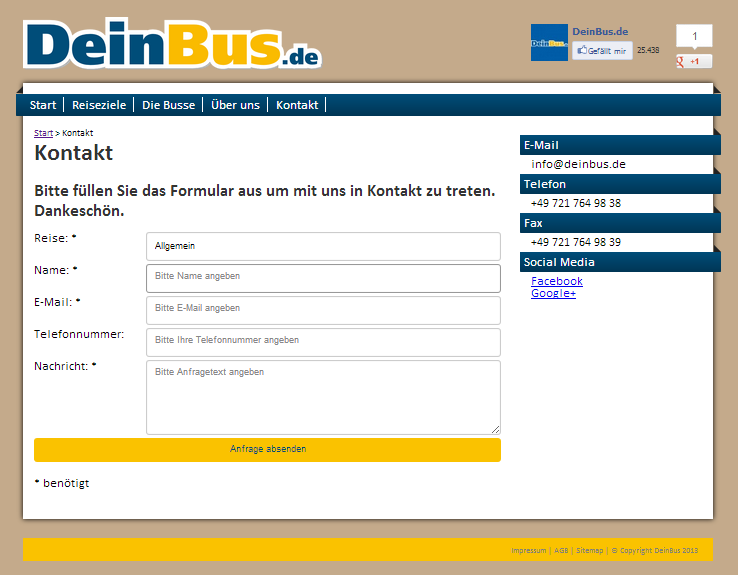
\includegraphics{scr_kontakt}
%Bitte Bild einf�gen, k.A. wie das geht :P

Die Seite "`Kontakt"' besteht zum gr��ten Teil aus einem Kontaktformular und den alternativen Kontaktm�glichkeiten in der Sidebar. 

Das Kontaktformular verwendet das �bliche HTML-Tag "`Form"' sowie einige HTML5-Funktionen. Erkennbar ist dies z.B. an dem Attribut "`required"', welches dem Browser signalisiert, dass dieses Formularelement ausgef�llt werden muss. Versucht der Benutzer das Formular abzuschicken erh�lt er einen Hinweis �ber das leere Element und wird aufgefordert es auszuf�llen - vorausgesetzt der Browser ist HTML5-kompatibel. Das Formular wird durch eine �bliche Tabelle strukturiert (table-tag).

%CODE 
/*...*/

			<tr>
				<td>Name: *</td>
				<td><input id="name" placeholder="Bitte Name angeben" type="text" tabindex="1" required autofocus></td>
			</tr>
/*...*/
%CODE Ende

F�r den Fall einer fehlenden HTML5-Unterst�tzung wurde eine Fallback-L�sung mittels JavaScript implementiert. Die Pr�fung auf eine HTML5-Unterst�tzung wurde wie folgt umgesetzt und wird bei jedem Abschicken des Formulars durchgef�hrt.

%CODE
/*...*/
	var inputs = document.createElement('input');
	var supports = {};
	supports.required  = 'required' in inputs;

	if(!supports.required) {
	/*...siehe unten...*/
	}
/*...*/
%CODE Ende

Trifft die Pr�fung zu und HTML5 wird nicht unterst�tzt wird jedes auszuf�llende Formularelement auf dessen Inhalt gepr�ft. Bei einem Fehler wird die Formular�bermittlung abgebrochen und der Fokus auf das betroffene Element gesetzt.

%CODE

/*...*/
		 name = document.getElementById("name").value;
/*...*/
		 if (name == "")
		 {
		 document.getElementById("name").select();
		 document.getElementById("name").focus();
		 return false;
		 }
/*...*/

%CODE ENDE

Da HTML5 auch die Plausibilit�t von E-Mail-Adressen pr�ft wurde auch dies im Fallback ber�cksichtigt. Hierf�r wurde ein Regul�rer Ausdruck verwendet:

%CODE
/*...*/
		 if (!checkEmail(email))
		 {
		 alert('E-Mail ist ung�ltig.');
		 return false;
		 }
/*...*/

function checkEmail(inputvalue) {
	var pattern = /^([a-zA-Z0-9_\.\-])+\@(([a-zA-Z0-9\-])+\.)+([a-zA-Z0-9]{2,4})+$/;
	return pattern.test(inputvalue);
}
/*...*/

%CODE ENDE